\documentclass[10pt,a4paper]{article}
\usepackage[margin=2.5cm]{geometry}
\usepackage{graphicx}
\usepackage{booktabs}
\usepackage{amsmath,amssymb}
\usepackage{hyperref}
\usepackage[numbers]{natbib}
\usepackage{subcaption}
\usepackage{xcolor}
\usepackage{float}
\usepackage{caption}
\hypersetup{colorlinks=true, linkcolor=blue, citecolor=blue, urlcolor=blue}

\title{\textbf{Advanced Few-Shot Flower Recognition:\\
A Comparison of CNN Modifications, Regularization, and Visual Prompt Tuning}}
\author{Jonas Tua \and Jia Ying Thor \and F Syed Abu Thahir}
\date{NTU SC4001 Sem 2 2026 \\ \today}

\begin{document}

\begin{titlepage}
\centering
\vspace*{2cm}
\includegraphics[width=0.5\textwidth]{figures/ntu-logo.png}\\
\vspace{3cm}
{\Huge\bfseries Advanced Few-Shot\\ Flower Recognition\par}
\vspace{1cm}
{\Large NTU SC4001 Sem 2 2026\par}
\vspace{2cm}
{\large Jonas Tua\qquad Jia Ying Thor\qquad F Syed Abu Thahir\par}
\vspace{4cm}
{\large \today\par}
\end{titlepage}

\begin{abstract}
We compare CNN architectures and Visual Prompt Tuning (VPT) for fine-grained flower classification on Oxford Flowers 102, where each class has only ten training images. Across eleven ResNet18 configurations, a ResNet50 baseline, and two VPT variants (Shallow and Deep), we measure how each method performs at $k \in \{1, 2, 5, 10\}$ images per class, using mean per-class accuracy as the primary metric following \citet{nilsback2008}.

We expected the advanced convolutions (dilated, deformable, depthwise-separable, and our novel hybrid) to outperform a plain ResNet18. None of them did. Regularization helped a bit: freezing the first two ResNet18 layers reaches 90.82\% mean per-class accuracy on the test set. MixUp, often a default regularizer, hurt performance under this data scale. The clear winner was VPT-Deep, reaching 92.83\% mean per-class accuracy while training only 0.2\% of the backbone parameters. The gap between VPT-Deep and full fine-tuning grows as the training budget shrinks.
\end{abstract}


\section{Introduction}
\subsection{Problem Motivation}

Fine-grained classification means telling apart visually similar categories: bird species, dog breeds, flower types. The model has to pick up on subtle differences in shape and colour while shrugging off variations in lighting and pose.

Oxford Flowers 102 \citep{nilsback2008} makes this harder by giving us very little to work with. The standard split has only 10 training images per class across 102 classes, which is barely enough to fit a softmax head, let alone an 11M-parameter network. That makes it a useful benchmark for few-shot methods.

CNNs and Vision Transformers (ViTs) do well on large datasets, but it is less obvious how they behave when training data is scarce. We wanted to find out which adaptation strategy holds up best at $k \in \{1, 2, 5, 10\}$ examples per class.

\subsection{Approach Overview}

We compare three families of adaptation under a single shared training recipe (AdamW, cosine annealing, 50 epochs, batch size 32) so that any difference in performance is attributable to the method itself:

\begin{itemize}
  \item \textbf{Five ResNet18 variants}: a baseline plus four advanced convolutional modifications (dilated, deformable, depthwise-separable, and our novel hybrid combining dilated and deformable layers).
  \item \textbf{Four regularization strategies} on top of the ResNet18 baseline: freezing early layers, label smoothing, MixUp, and stronger image augmentation.
  \item \textbf{A larger CNN backbone} (ResNet50) to test whether more capacity helps.
  \item \textbf{Visual Prompt Tuning (VPT)} on a ViT-B/16 backbone, in both Shallow and Deep configurations \citep{jia2022vpt}.
\end{itemize}

We measure accuracy, mean per-class accuracy, and top-5 accuracy on the test set. We also rerun every method at $k = 1, 2, 5$ images per class to see how it degrades. Two questions drive the work: does architectural complexity actually help in the few-shot regime, and can parameter-efficient tuning match or beat full fine-tuning on a fine-grained task?

\subsection{Training and Evaluation Setup}

We use the canonical \texttt{torchvision.datasets.Flowers102} split: 1020 training images, 1020 validation images, and 6149 test images. Images are resized to $224 \times 224$ and normalised with ImageNet statistics. The training transform applies a random horizontal flip and rotation up to 15 degrees.

We report three test-set metrics:
\begin{itemize}
  \item \textbf{Accuracy}: overall correct predictions over all samples.
  \item \textbf{Mean per-class accuracy (MPC)}: average per-class recall, our primary metric following \citet{nilsback2008}. The test set is class-imbalanced (20 to 258 images per class), so this corrects for class frequency.
  \item \textbf{Top-5 accuracy}: fraction of samples where the true class appears in the top-5 predictions.
\end{itemize}

Unless stated otherwise, every model trains for 50 epochs with AdamW ($\text{lr} = 10^{-3}$), cosine annealing, batch size 32, automatic mixed precision, and seed 69. Experiments run on a single NVIDIA RTX 3070 Ti.


\section{Baseline: ResNet18 Transfer Learning}
We start with the simplest recipe that still leverages pre-training: take a ResNet18 pre-trained on ImageNet-1k, replace the final classification layer with a 102-way linear head, and fine-tune every parameter. This baseline tells us what standard transfer learning gets without tricks.

\subsection{Architecture}
We use \texttt{torchvision.models.resnet18} with \texttt{ResNet18\_Weights.DEFAULT}. The original 1000-way classifier is replaced with \texttt{nn.Linear(512, 102)}. All weights are trainable. The model has 11,228,838 parameters, matching the standard ResNet18.

\subsection{Results and Analysis}
The baseline reaches 86.11\% mean per-class accuracy on the test set (Table~\ref{tab:main-results}). Training accuracy reaches 100\% before epoch 20, while validation accuracy plateaus near 88\%, a gap of more than ten points that signals overfitting. With ten images per class spread over 102 classes, the model simply memorises the training set. The confusion matrix (analysed for the best model in \S\ref{sec:discussion}) shows the baseline struggles most on classes with high intra-class variability like ``bolero deep blue'' and ``common dandelion'', where different lighting or pose produces visibly different images of the same flower.

This baseline sets the floor for what the rest of the report improves on (or fails to improve on).


\section{Advanced Convolution Techniques}
Flower classification benefits from features at multiple spatial scales: petal shape requires local geometry, while overall arrangement requires a wider receptive field. We test whether replacing the standard $3 \times 3$ convolution with a more expressive operator helps ResNet18 learn better features for this task. All variants in this section preserve the pre-trained weights by copying them into the new operator where the shapes allow.

\subsection{Dilated Convolution}
Dilated convolution \citep{yu2016dilated} inserts zeros between kernel weights, enlarging the receptive field without adding parameters. A $k \times k$ kernel with dilation rate $d$ has effective receptive field
\[
  RF = k + (k-1)(d-1).
\]
We replace every $3 \times 3$ convolution in \texttt{layer3} and \texttt{layer4} with a dilation-2 version and copy the pre-trained weights into the new layer (the weight tensor shape is unchanged).

\subsection{Deformable Convolution}
Deformable convolution \citep{dai2017deformable} learns a per-pixel offset $\Delta p$ for each kernel position, shifting the sampling grid to follow object geometry. We implement the v1 variant with \texttt{torchvision.ops.deform\_conv2d}. A small auxiliary convolution predicts the offsets, initialised to zero so that the module starts as a standard convolution. As with dilation, we copy pre-trained weights into the main kernel and only the offset predictor is new. We apply this to the first $3 \times 3$ convolution in each BasicBlock of \texttt{layer3} and \texttt{layer4}.

\subsection{Depthwise-Separable Convolution}
Depthwise-separable convolution \citep{howard2017mobilenets} factors a standard convolution into a depthwise spatial filter (one kernel per channel) followed by a pointwise $1 \times 1$ mixing. This cuts the parameter count from $C_{\text{in}} \cdot C_{\text{out}} \cdot k^2$ to $C_{\text{in}} \cdot k^2 + C_{\text{in}} \cdot C_{\text{out}}$. We replace every $3 \times 3$ convolution in \texttt{layer2}, \texttt{layer3}, and \texttt{layer4}. The weight shapes change, so pre-trained initialisation is not possible.

\subsection{Novel Hybrid: Dilated + Deformable}
We combine the two strategies that preserve pre-trained weights. Dilated convolutions go in \texttt{layer3} (wider receptive field at mid-level features), and deformable convolutions go in \texttt{layer4} (input-adaptive sampling at the highest semantic level). To our knowledge, this specific combination has not been reported in the flower classification literature.

\subsection{Results and Analysis}
All four variants underperform the baseline (Table~\ref{tab:main-results}). The best of the four is deformable convolution at 83.46\% MPC accuracy (baseline: 86.11\%); the worst is depthwise-separable at 59.71\%. The hybrid variant (81.34\%) falls between dilated (78.53\%) and deformable, without outperforming either component alone.

\begin{table}[H]
\centering
\small
\begin{tabular}{lcc}
\toprule
Method & MPC Acc (\%) & Test Acc (\%) \\
\midrule
Baseline (unmodified) & \textbf{86.11} & \textbf{84.42} \\
+ Deformable conv     & 83.46 & 81.33 \\
+ Hybrid (dilated+deformable) & 81.34 & 78.73 \\
+ Dilated conv        & 78.53 & 75.95 \\
+ Depthwise-separable & 59.71 & 57.03 \\
\bottomrule
\end{tabular}
\caption{Advanced convolution techniques on ResNet18. None match the unmodified baseline.}
\label{tab:conv-results}
\end{table}

Three factors explain this outcome. First, the pre-trained weights were learned for standard convolution; replacing the operator introduces a mismatch between the weights and the computation. Dilation spreads the kernel sampling across a wider region, which the original weights were not calibrated for. Second, the offset predictor in deformable convolution starts at zero and gradually learns useful displacements, but with only 1020 training images it never gets a strong enough signal. Third, depthwise-separable convolution simply cannot reuse the pre-trained weights (different tensor shape), so it starts from scratch and fails to make up the gap in 50 epochs.

Our novel hybrid does not beat either component. The signal we take from this section is that modifying the convolutional operator is the wrong lever to pull when pre-trained features are strong and training data is scarce.


\section{Regularization Techniques}
The baseline overfits (100\% train accuracy, 86\% MPC test accuracy). If the bottleneck is overfitting rather than architecture, regularization should help. We test four regularizers while keeping the ResNet18 architecture fixed.

\subsection{Freezing Early Layers}
The pre-trained weights in \texttt{layer1} and \texttt{layer2} encode low-level features (edges, textures) that transfer well across datasets. Freezing them reduces the trainable parameter count from 11.2M to 10.5M and prevents the low-level features from drifting during fine-tuning. Only \texttt{layer3}, \texttt{layer4}, and the classifier head receive gradient updates.

\subsection{Label Smoothing}
Label smoothing \citep{szegedy2016rethinking} replaces the one-hot target $y$ with a softened target
\[
  \tilde{y}_i = (1-\alpha) \cdot y_i + \alpha / K,
\]
where $K$ is the number of classes. We set $\alpha = 0.1$. This prevents the logits from growing arbitrarily large and reduces overconfidence on the training set. We change one line: \texttt{nn.CrossEntropyLoss(label\_smoothing=0.1)}.

\subsection{MixUp Augmentation}
MixUp \citep{zhang2018mixup} trains on convex combinations of image and label pairs:
\[
  \tilde{x} = \lambda x_i + (1-\lambda) x_j, \qquad \tilde{y} = \lambda y_i + (1-\lambda) y_j,
\]
with $\lambda \sim \text{Beta}(\alpha, \alpha)$. We use the official \texttt{torchvision.transforms.v2.MixUp} implementation via a DataLoader \texttt{collate\_fn} with $\alpha = 0.2$.

\subsection{Stronger Data Augmentation}
The default augmentation pipeline is mild (horizontal flip plus small rotation). We also train with a stronger pipeline: \texttt{RandomResizedCrop(scale=(0.6, 1.0))} and \texttt{ColorJitter(brightness=0.2, contrast=0.2, saturation=0.2, hue=0.1)}.

\subsection{Results and Analysis}
Table~\ref{tab:reg-results} shows that three of four regularizers help, but only marginally, and one (MixUp) actively hurts.

\begin{table}[H]
\centering
\small
\begin{tabular}{lcc}
\toprule
Method & MPC Acc (\%) & $\Delta$ vs.\ baseline \\
\midrule
Frozen layer1+2       & \textbf{90.82} & +4.71 \\
Label smoothing ($\alpha{=}0.1$) & 89.40 & +3.29 \\
Label smoothing + strong aug & 88.24 & +2.13 \\
Baseline              & 86.11 & --- \\
Strong aug only       & 86.11 & +0.00 \\
MixUp ($\alpha{=}0.2$) & 83.50 & $-2.61$ \\
\bottomrule
\end{tabular}
\caption{Regularization techniques on ResNet18.}
\label{tab:reg-results}
\end{table}

Freezing the first two layers gives the largest gain and pushes MPC accuracy to 90.82\%, a 4.7-point improvement at the cost of only 6\% fewer trainable parameters. Label smoothing adds another useful 3 points on top of the baseline, though combining it with strong augmentation does worse than label smoothing alone, suggesting the two tools compete for the same regularization budget.

MixUp is the surprise. In most image classification settings it improves generalisation, but here it drops MPC accuracy by 2.6 points. We suspect two reasons. With ten images per class and 102 classes, many mixed pairs span visually unrelated species, and the resulting soft labels provide little discriminative signal. And the model already overfits on unmixed examples, so spending capacity to memorise blends leaves less for the clean examples at test time. Stronger augmentation on its own gives the same MPC accuracy as the baseline, which we read as the dataset already being tolerant to mild geometric variation.

The pattern in this section points in the same direction as \S3: the most useful thing we did was \emph{not train} part of the network (freezing layer1 and layer2). This primes the argument for Visual Prompt Tuning, which is the extreme version of the same idea.


\section{Scaling the Backbone: ResNet50}
Does a bigger backbone help? We swap ResNet18 (11.2M parameters) for ResNet50 (23.7M) and fine-tune the full network under the same recipe as the baseline. ResNet50 has been reported to reach 91--97\% on Flowers 102 in recent work, often with additional tricks.

\subsection{Results and Analysis}
ResNet50 reaches 88.07\% MPC accuracy on the test set, only two points above our ResNet18 baseline and well below the frozen-layers ResNet18 (90.82\%). The gain from doubling the parameter count is smaller than the gain from simply freezing the first two layers of a smaller model.

We read this as evidence that the ten-shot Flowers 102 budget is too small to exploit the extra capacity of ResNet50. The larger model has more parameters to overfit, and our training recipe does not include the aggressive augmentation or longer schedules that reported high ResNet50 numbers typically rely on. Scaling up the backbone is not cost-free on this dataset.


\section{Visual Prompt Tuning}
Sections \S3--\S5 all share one property: they modify or fine-tune a pre-trained network's weights. Visual Prompt Tuning \citep{jia2022vpt} does something different. It freezes the entire backbone and inserts a small set of learnable \emph{prompt tokens} into the input space of a Vision Transformer, training only those prompts plus the classifier head. We test both variants from the original paper.

\subsection{VPT-Shallow}
VPT-Shallow inserts prompts only at the first Transformer layer. Given an image embedded into patch tokens $E_0 = [e_0^1, \dots, e_0^m]$ and a classification token $x_0$, VPT-Shallow prepends $p$ learnable prompts $P = [\mathbf{p}^1, \dots, \mathbf{p}^p]$:
\[
  [x_1, Z_1, E_1] = L_1([x_0, P, E_0]),
\]
where $L_1$ is the first frozen Transformer layer and $Z_1$ are the processed prompt outputs (discarded). The remaining layers receive $[x_i, Z_i, E_i]$ unchanged. Only $P$ and the classifier head are trained.

We use ViT-B/16 pre-trained on ImageNet-1k as the backbone and $p = 10$ prompts. Trainable parameter count: 86,118.

\subsection{VPT-Deep}
VPT-Deep inserts fresh prompts at \emph{every} Transformer layer:
\[
  [x_i, \_, E_i] = L_i([x_{i-1}, P_{i-1}, E_{i-1}]),
\]
where $P_{i-1}$ is a layer-specific learnable prompt matrix. The prompts from the previous layer are discarded at each step, so only $P_0, \dots, P_{N-1}$ and the classifier head are trained. With $p = 10$ and 12 Transformer layers, the model has 170,598 trainable parameters, which is 0.2\% of the ViT-B/16 backbone.

\subsection{Results and Analysis}
\begin{table}[H]
\centering
\small
\begin{tabular}{lcccc}
\toprule
Method & Test Acc (\%) & MPC Acc (\%) & Top-5 (\%) & Trainable params \\
\midrule
VPT-Deep    & \textbf{91.64} & \textbf{92.83} & \textbf{97.93} & 170,598 \\
VPT-Shallow & 84.13 & 85.70 & 95.43 & 86,118 \\
Frozen ResNet18 (best CNN) & 88.52 & 90.82 & --- & 10,545,766 \\
\bottomrule
\end{tabular}
\caption{Visual Prompt Tuning versus the best CNN we tuned.}
\label{tab:vpt-results}
\end{table}

VPT-Deep beats every CNN configuration we trained, including the frozen-layer ResNet18 that won \S4. It does so with 62$\times$ fewer trainable parameters than the frozen ResNet18 and 139$\times$ fewer than full ResNet18 fine-tuning. Top-5 accuracy of 97.93\% means the correct class is among the top five predictions for all but 2\% of test images.

VPT-Shallow (85.70\% MPC) is competitive with the unmodified ResNet18 baseline (86.11\%) but falls short of the best CNN. This matches the pattern reported in the original VPT paper: shallow prompts alone do not provide enough capacity for fine-grained recognition, and inserting prompts at every layer is worth the extra 85K parameters.

\textbf{Prompt length ablation.} Figure~\ref{fig:prompt-length} varies the number of prompts per layer for VPT-Deep. Accuracy increases monotonically from $p=1$ (91.08\% val) to $p=50$ (94.51\% val). Our default $p=10$ gives 93.63\%. Longer prompts continue to help, but with diminishing returns and more parameters.

\begin{figure}[H]
\centering
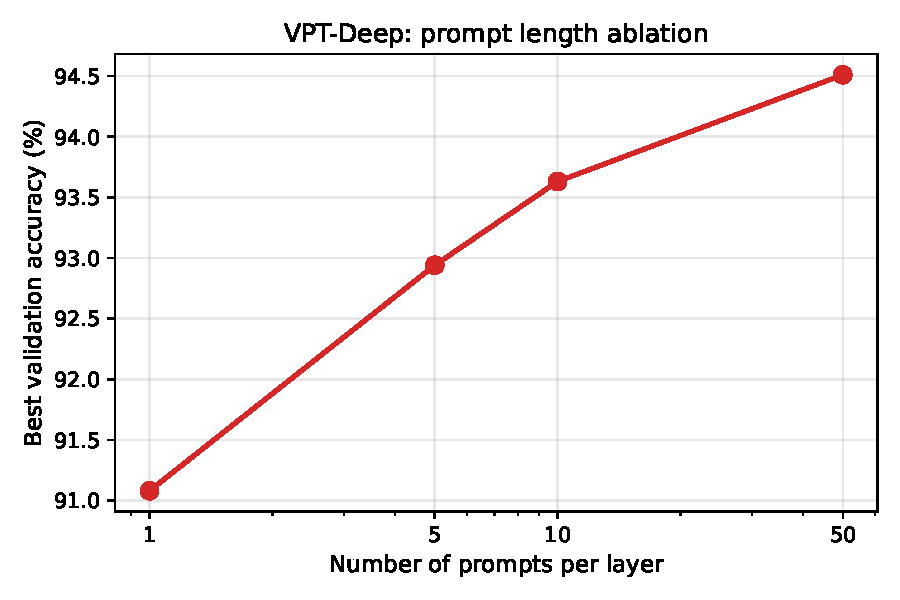
\includegraphics[width=0.65\textwidth]{figures/prompt-length.pdf}
\caption{VPT-Deep accuracy vs.\ number of prompts per layer.}
\label{fig:prompt-length}
\end{figure}


\section{Few-Shot Learning Analysis}
The default Flowers 102 split is already low-data (ten images per class). We test how each method behaves as the training budget shrinks further, which is the setting where parameter-efficient tuning should help most.

\subsection{Experimental Setup}
For $k \in \{1, 2, 5\}$, we subsample the training set to $k$ images per class (first $k$ per class, deterministic with seed 69). The validation and test sets are unchanged. We train for 30 epochs (shorter because the dataset is smaller) with the same optimizer and schedule as the full-data experiments. We use the same six methods for every $k$.

\subsection{Results and Analysis}
Figure~\ref{fig:fewshot} plots the best validation accuracy at each $k$.

\begin{figure}[H]
\centering
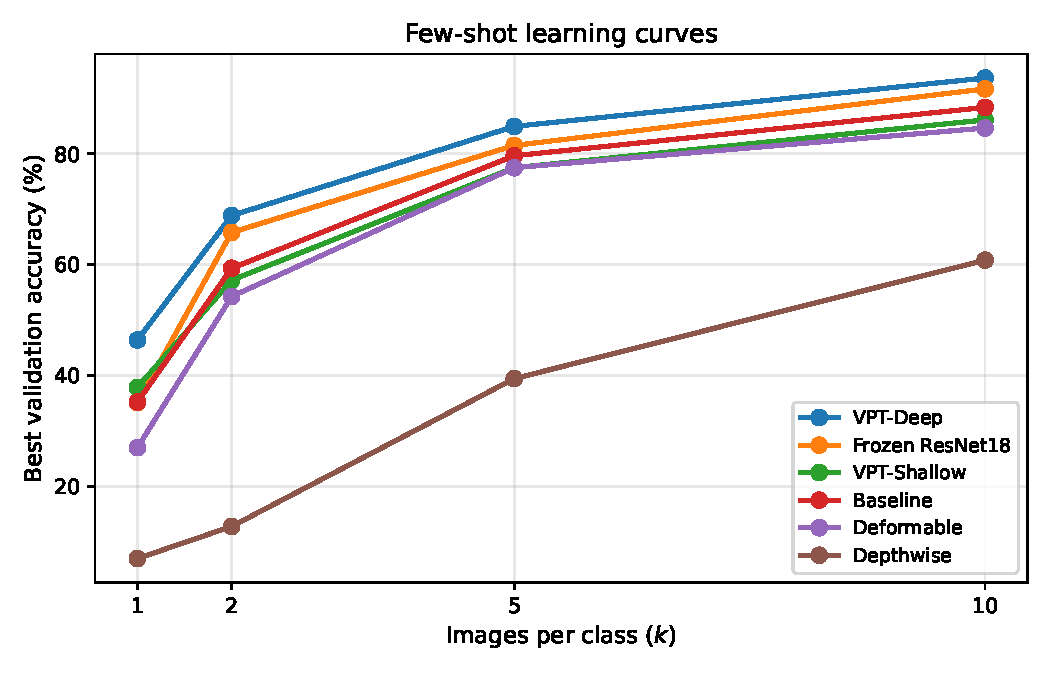
\includegraphics[width=0.75\textwidth]{figures/fewshot-curves.pdf}
\caption{Few-shot learning curves. VPT-Deep dominates across all $k$.}
\label{fig:fewshot}
\end{figure}

\begin{table}[H]
\centering
\small
\begin{tabular}{lcccc}
\toprule
Method & $k{=}1$ & $k{=}2$ & $k{=}5$ & $k{=}10$ \\
\midrule
VPT-Deep           & \textbf{46.37} & \textbf{68.82} & \textbf{84.90} & \textbf{93.63} \\
Frozen ResNet18    & 35.10 & 65.78 & 81.47 & 91.67 \\
VPT-Shallow        & 37.84 & 57.16 & 77.45 & 86.08 \\
Baseline (full FT) & 35.20 & 59.31 & 79.61 & 88.33 \\
Deformable         & 26.96 & 54.22 & 77.45 & 84.61 \\
Depthwise          & 6.96  & 12.75 & 39.41 & 60.78 \\
\bottomrule
\end{tabular}
\caption{Best validation accuracy (\%) at different training budgets.}
\label{tab:fewshot}
\end{table}

VPT-Deep wins at every $k$. The margin over the frozen ResNet18 is roughly one point at $k=10$, three points at $k=5$, three points at $k=2$, and eleven points at $k=1$. Low-data regimes widen the gap, which matches the central message of \citet{jia2022vpt}: with fewer labelled examples, updating fewer parameters is the right move. The baseline (which fine-tunes 11M parameters) sits below both VPT and the frozen ResNet18 at small $k$, and catches up only at $k=10$.

Depthwise-separable collapses at low $k$ (6.96\% at $k=1$) because it starts from randomly initialised weights and cannot recover with so few examples. Deformable convolution is also hurt at small $k$: the offset predictor needs more data to learn useful displacements than is available.

Put together with Table~\ref{tab:main-results}, the few-shot curves are the strongest version of our thesis: the less data you have, the more you should lean on pre-trained features, and the less you should modify the backbone.


\section{Discussion}
\label{sec:discussion}

Table~\ref{tab:main-results} and Figure~\ref{fig:param-efficiency} together summarise the experiments. The parameter efficiency scatter is the single visual that captures our thesis.

\begin{table}[H]
\centering
\small
\begin{tabular}{lccc r}
\toprule
Method & Test Acc (\%) & MPC Acc (\%) & Top-5 (\%) & Trainable params \\
\midrule
\textbf{VPT-Deep}           & \textbf{91.64} & \textbf{92.83} & \textbf{97.93} & \textbf{170{,}598} \\
Frozen ResNet18             & 88.52 & 90.82 & --- & 10{,}545{,}766 \\
Label smoothing             & 87.27 & 89.40 & --- & 11{,}228{,}838 \\
ResNet50                    & 85.93 & 88.07 & --- & 23{,}717{,}030 \\
VPT-Shallow                 & 84.13 & 85.70 & 95.43 & 86{,}118 \\
Baseline                    & 84.42 & 86.11 & --- & 11{,}228{,}838 \\
Deformable                  & 81.33 & 83.46 & --- & 11{,}415{,}534 \\
MixUp                       & 80.52 & 83.50 & --- & 11{,}228{,}838 \\
Hybrid (ours)               & 78.73 & 81.34 & --- & 11{,}353{,}290 \\
Dilated                     & 75.95 & 78.53 & --- & 11{,}228{,}838 \\
Depthwise                   & 57.03 & 59.71 & --- & 1{,}623{,}270 \\
\bottomrule
\end{tabular}
\caption{Test-set results for every model we trained, sorted by mean per-class accuracy.}
\label{tab:main-results}
\end{table}

\begin{figure}[H]
\centering
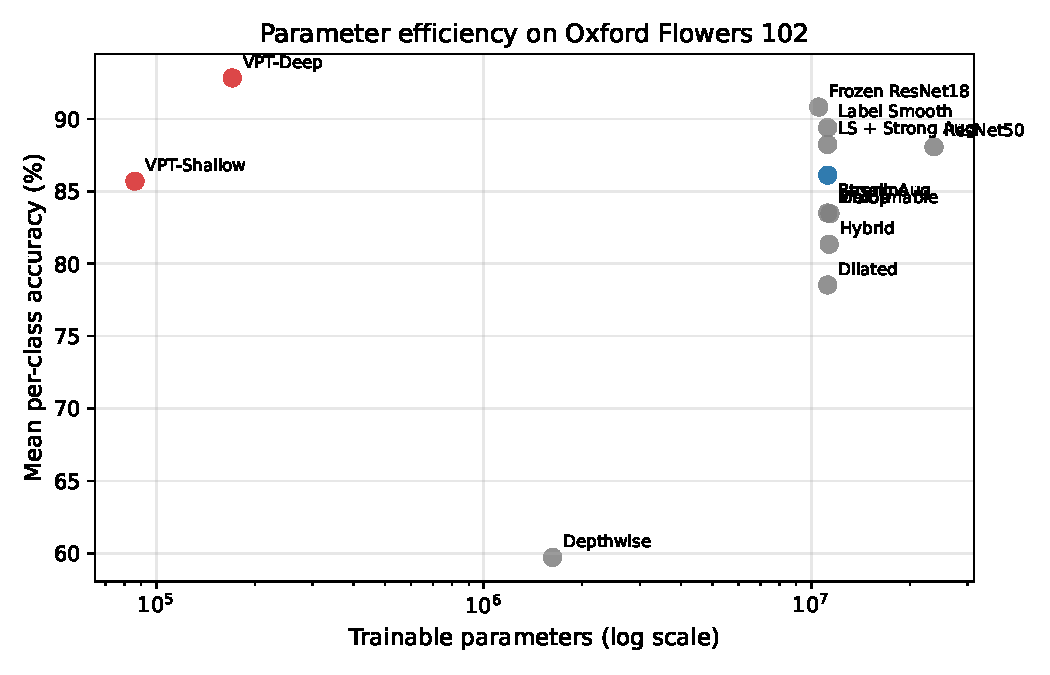
\includegraphics[width=0.8\textwidth]{figures/parameter-efficiency.pdf}
\caption{Mean per-class accuracy versus trainable parameter count. VPT variants sit in the top-left corner (best accuracy at smallest parameter count). CNN variants occupy the middle-right region.}
\label{fig:param-efficiency}
\end{figure}

\textbf{What worked.} VPT-Deep outperformed every CNN configuration we trained. Freezing the first two ResNet18 layers was the most useful CNN intervention. Label smoothing gave a small but cheap improvement. Scaling to ResNet50 produced a modest gain that did not justify its extra cost.

\textbf{What did not work, and why.} Four findings went against common defaults:

\emph{Dilated, deformable, and hybrid convolutions hurt.} All four convolutional modifications we tested dropped MPC accuracy below the baseline, despite being well-motivated on paper. The shared cause is the mismatch between the pre-trained weights and the new operator. Dilation spreads the sampling grid across a wider area than the weights were trained for. The deformable offset predictor starts from a zero initialisation and needs more data than 1020 images to learn useful offsets.

\emph{Depthwise-separable convolution collapses.} With the kernel shape changed, pre-trained weights cannot be copied and the model learns from scratch. Fifty epochs of 1020 images are not enough to make this viable.

\emph{MixUp hurts at ten shots per class.} MixUp is a default regularizer in most vision pipelines, but under extreme data scarcity it damages performance. With 102 classes and 10 examples each, most mixed pairs cross unrelated species, and the resulting soft labels carry little class-discriminative signal.

\emph{Strong augmentation alone does not help.} RandomResizedCrop and ColorJitter together produced the same MPC accuracy as the baseline, suggesting Flowers 102 already tolerates mild geometric variation and that the true bottleneck is overfitting to class identity, not to pose.

\textbf{Why VPT-Deep wins.} Two forces compound. First, its parameter budget is 60 to 140 times smaller than the CNN alternatives, which limits overfitting. Second, it never disturbs the pre-trained backbone. The learnable prompts act as task-specific queries that reshape the input distribution seen by the frozen Transformer layers, without asking those layers to change what they computed on ImageNet-21k. Few-shot results make the second point concrete: the gap between VPT-Deep and the best CNN widens as training data shrinks, because the CNN has more parameters to spoil and fewer examples to constrain them.

\textbf{Comparison to prior work.} \citet{nilsback2008} reported 72.8\% accuracy with hand-engineered features and a multiple-kernel SVM. Our VPT-Deep result (91.64\% test accuracy) is consistent with the general Transformer-based numbers from recent work, though direct comparison is difficult because many recent papers use larger backbones (ViT-L/14), additional tricks, or different train/test splits. \citet{jia2022vpt} reported 89.11\% average across five FGVC datasets for VPT-Deep on a ViT-B/16 pre-trained on ImageNet-21k; our 92.83\% MPC on ImageNet-1k pre-trained weights sits above that average.

\textbf{Limitations.} We evaluate a single seed and a single backbone. Variance across seeds is an obvious gap. We also did not implement triplet loss (noted as a future-work suggestion in the project handout) or test-time augmentation, both of which could push the numbers higher. The prompt length ablation (Figure~\ref{fig:prompt-length}) shows that $p=50$ beats our $p=10$ default, so the VPT-Deep results reported in Table~\ref{tab:main-results} are not the best the method can do.


\section{Conclusion}
We compared three families of adaptation on Oxford Flowers 102: architectural modification (dilated, deformable, depthwise-separable, hybrid convolutions), training-time regularization (frozen layers, label smoothing, MixUp, strong augmentation), and parameter-efficient tuning (Visual Prompt Tuning, shallow and deep). Across 13 training runs and a few-shot sweep at $k \in \{1, 2, 5, 10\}$, VPT-Deep came out ahead, reaching 92.83\% mean per-class accuracy on the test set while updating only 0.2\% of the backbone parameters.

The central finding is that fine-grained classification with limited data rewards parameter efficiency more than architectural cleverness. Modifying the convolutional operator consistently hurt performance. The most useful thing we did to the CNN was freeze its early layers, which is the same logic that drives VPT to its extreme: do not touch the pre-trained weights at all.

Two results surprised us. MixUp, a near-default regularizer in modern image classification, dropped accuracy by 2.6 points at ten shots per class because mixing rarely preserves class-discriminative information at that data scale. Scaling the backbone from ResNet18 to ResNet50 gave a smaller gain than simply freezing the first two layers of the smaller model, which argues that capacity is not the bottleneck.

Future work would integrate triplet loss into the VPT recipe, test VPT at larger prompt lengths with longer training, and measure variance across random seeds. The main limitation of this report is that every number reflects a single run.


\bibliographystyle{unsrtnat}
\bibliography{bibliography}

\end{document}
